% Options for packages loaded elsewhere
\PassOptionsToPackage{unicode}{hyperref}
\PassOptionsToPackage{hyphens}{url}
%
\documentclass[
]{article}
\usepackage{amsmath,amssymb}
\usepackage{iftex}
\ifPDFTeX
  \usepackage[T1]{fontenc}
  \usepackage[utf8]{inputenc}
  \usepackage{textcomp} % provide euro and other symbols
\else % if luatex or xetex
  \usepackage{unicode-math} % this also loads fontspec
  \defaultfontfeatures{Scale=MatchLowercase}
  \defaultfontfeatures[\rmfamily]{Ligatures=TeX,Scale=1}
\fi
\usepackage{lmodern}
\ifPDFTeX\else
  % xetex/luatex font selection
\fi
% Use upquote if available, for straight quotes in verbatim environments
\IfFileExists{upquote.sty}{\usepackage{upquote}}{}
\IfFileExists{microtype.sty}{% use microtype if available
  \usepackage[]{microtype}
  \UseMicrotypeSet[protrusion]{basicmath} % disable protrusion for tt fonts
}{}
\makeatletter
\@ifundefined{KOMAClassName}{% if non-KOMA class
  \IfFileExists{parskip.sty}{%
    \usepackage{parskip}
  }{% else
    \setlength{\parindent}{0pt}
    \setlength{\parskip}{6pt plus 2pt minus 1pt}}
}{% if KOMA class
  \KOMAoptions{parskip=half}}
\makeatother
\usepackage{xcolor}
\usepackage[margin=1in]{geometry}
\usepackage{color}
\usepackage{fancyvrb}
\newcommand{\VerbBar}{|}
\newcommand{\VERB}{\Verb[commandchars=\\\{\}]}
\DefineVerbatimEnvironment{Highlighting}{Verbatim}{commandchars=\\\{\}}
% Add ',fontsize=\small' for more characters per line
\usepackage{framed}
\definecolor{shadecolor}{RGB}{248,248,248}
\newenvironment{Shaded}{\begin{snugshade}}{\end{snugshade}}
\newcommand{\AlertTok}[1]{\textcolor[rgb]{0.94,0.16,0.16}{#1}}
\newcommand{\AnnotationTok}[1]{\textcolor[rgb]{0.56,0.35,0.01}{\textbf{\textit{#1}}}}
\newcommand{\AttributeTok}[1]{\textcolor[rgb]{0.13,0.29,0.53}{#1}}
\newcommand{\BaseNTok}[1]{\textcolor[rgb]{0.00,0.00,0.81}{#1}}
\newcommand{\BuiltInTok}[1]{#1}
\newcommand{\CharTok}[1]{\textcolor[rgb]{0.31,0.60,0.02}{#1}}
\newcommand{\CommentTok}[1]{\textcolor[rgb]{0.56,0.35,0.01}{\textit{#1}}}
\newcommand{\CommentVarTok}[1]{\textcolor[rgb]{0.56,0.35,0.01}{\textbf{\textit{#1}}}}
\newcommand{\ConstantTok}[1]{\textcolor[rgb]{0.56,0.35,0.01}{#1}}
\newcommand{\ControlFlowTok}[1]{\textcolor[rgb]{0.13,0.29,0.53}{\textbf{#1}}}
\newcommand{\DataTypeTok}[1]{\textcolor[rgb]{0.13,0.29,0.53}{#1}}
\newcommand{\DecValTok}[1]{\textcolor[rgb]{0.00,0.00,0.81}{#1}}
\newcommand{\DocumentationTok}[1]{\textcolor[rgb]{0.56,0.35,0.01}{\textbf{\textit{#1}}}}
\newcommand{\ErrorTok}[1]{\textcolor[rgb]{0.64,0.00,0.00}{\textbf{#1}}}
\newcommand{\ExtensionTok}[1]{#1}
\newcommand{\FloatTok}[1]{\textcolor[rgb]{0.00,0.00,0.81}{#1}}
\newcommand{\FunctionTok}[1]{\textcolor[rgb]{0.13,0.29,0.53}{\textbf{#1}}}
\newcommand{\ImportTok}[1]{#1}
\newcommand{\InformationTok}[1]{\textcolor[rgb]{0.56,0.35,0.01}{\textbf{\textit{#1}}}}
\newcommand{\KeywordTok}[1]{\textcolor[rgb]{0.13,0.29,0.53}{\textbf{#1}}}
\newcommand{\NormalTok}[1]{#1}
\newcommand{\OperatorTok}[1]{\textcolor[rgb]{0.81,0.36,0.00}{\textbf{#1}}}
\newcommand{\OtherTok}[1]{\textcolor[rgb]{0.56,0.35,0.01}{#1}}
\newcommand{\PreprocessorTok}[1]{\textcolor[rgb]{0.56,0.35,0.01}{\textit{#1}}}
\newcommand{\RegionMarkerTok}[1]{#1}
\newcommand{\SpecialCharTok}[1]{\textcolor[rgb]{0.81,0.36,0.00}{\textbf{#1}}}
\newcommand{\SpecialStringTok}[1]{\textcolor[rgb]{0.31,0.60,0.02}{#1}}
\newcommand{\StringTok}[1]{\textcolor[rgb]{0.31,0.60,0.02}{#1}}
\newcommand{\VariableTok}[1]{\textcolor[rgb]{0.00,0.00,0.00}{#1}}
\newcommand{\VerbatimStringTok}[1]{\textcolor[rgb]{0.31,0.60,0.02}{#1}}
\newcommand{\WarningTok}[1]{\textcolor[rgb]{0.56,0.35,0.01}{\textbf{\textit{#1}}}}
\usepackage{graphicx}
\makeatletter
\def\maxwidth{\ifdim\Gin@nat@width>\linewidth\linewidth\else\Gin@nat@width\fi}
\def\maxheight{\ifdim\Gin@nat@height>\textheight\textheight\else\Gin@nat@height\fi}
\makeatother
% Scale images if necessary, so that they will not overflow the page
% margins by default, and it is still possible to overwrite the defaults
% using explicit options in \includegraphics[width, height, ...]{}
\setkeys{Gin}{width=\maxwidth,height=\maxheight,keepaspectratio}
% Set default figure placement to htbp
\makeatletter
\def\fps@figure{htbp}
\makeatother
\setlength{\emergencystretch}{3em} % prevent overfull lines
\providecommand{\tightlist}{%
  \setlength{\itemsep}{0pt}\setlength{\parskip}{0pt}}
\setcounter{secnumdepth}{-\maxdimen} % remove section numbering
\usepackage{fvextra}
\DefineVerbatimEnvironment{Highlighting}{Verbatim}{breaklines,commandchars=\\\{\}}
\ifLuaTeX
  \usepackage{selnolig}  % disable illegal ligatures
\fi
\usepackage{bookmark}
\IfFileExists{xurl.sty}{\usepackage{xurl}}{} % add URL line breaks if available
\urlstyle{same}
\hypersetup{
  pdftitle={SDA Group Submission Assignment Assign2},
  pdfauthor={MengliFeng (2720589) and PepijnVanOostveen (2801582)},
  hidelinks,
  pdfcreator={LaTeX via pandoc}}

\title{SDA Group Submission Assignment Assign2}
\usepackage{etoolbox}
\makeatletter
\providecommand{\subtitle}[1]{% add subtitle to \maketitle
  \apptocmd{\@title}{\par {\large #1 \par}}{}{}
}
\makeatother
\subtitle{Group Gr18}
\author{MengliFeng (2720589) and PepijnVanOostveen (2801582)}
\date{}

\begin{document}
\maketitle

\section{Exercise 1}\label{exercise-1}

\subsection{a.}\label{a.}

\begin{Shaded}
\begin{Highlighting}[]
\CommentTok{\# Set up a 2×3 grid for plotting (fills row{-}wise)}
\FunctionTok{par}\NormalTok{(}\AttributeTok{mfrow =} \FunctionTok{c}\NormalTok{(}\DecValTok{2}\NormalTok{, }\DecValTok{3}\NormalTok{), }\AttributeTok{mar =} \FunctionTok{c}\NormalTok{(}\DecValTok{4}\NormalTok{, }\DecValTok{4}\NormalTok{, }\DecValTok{2}\NormalTok{, }\DecValTok{1}\NormalTok{), }\AttributeTok{oma =} \FunctionTok{c}\NormalTok{(}\DecValTok{0}\NormalTok{, }\DecValTok{0}\NormalTok{, }\DecValTok{2}\NormalTok{, }\DecValTok{0}\NormalTok{))}

\CommentTok{\# Define probability points}
\NormalTok{p }\OtherTok{\textless{}{-}} \FunctionTok{seq}\NormalTok{(}\FloatTok{0.01}\NormalTok{, }\FloatTok{0.99}\NormalTok{, }\AttributeTok{length.out =} \DecValTok{100}\NormalTok{)}

\CommentTok{\# {-}{-}{-}{-} First Row: QQ{-}Plots {-}{-}{-}{-}}
\CommentTok{\# 1. QQ{-}Plot: t(3) vs Normal(0,2)}
\NormalTok{q\_t3 }\OtherTok{\textless{}{-}} \FunctionTok{qt}\NormalTok{(p, }\AttributeTok{df =} \DecValTok{3}\NormalTok{)}
\NormalTok{q\_norm }\OtherTok{\textless{}{-}} \FunctionTok{qnorm}\NormalTok{(p, }\AttributeTok{mean =} \DecValTok{0}\NormalTok{, }\AttributeTok{sd =} \FunctionTok{sqrt}\NormalTok{(}\DecValTok{2}\NormalTok{))}
\FunctionTok{plot}\NormalTok{(q\_t3, q\_norm, }\AttributeTok{type =} \StringTok{"l"}\NormalTok{, }\AttributeTok{xlab =} \StringTok{"t(3)"}\NormalTok{, }\AttributeTok{ylab =} \StringTok{"N(0,2)"}\NormalTok{)}

\CommentTok{\# 2. QQ{-}Plot: Chi{-}squared(25) vs Chi{-}squared(4)}
\NormalTok{q\_chisq25 }\OtherTok{\textless{}{-}} \FunctionTok{qchisq}\NormalTok{(p, }\AttributeTok{df =} \DecValTok{25}\NormalTok{)}
\NormalTok{q\_chisq4 }\OtherTok{\textless{}{-}} \FunctionTok{qchisq}\NormalTok{(p, }\AttributeTok{df =} \DecValTok{4}\NormalTok{)}
\FunctionTok{plot}\NormalTok{(q\_chisq25, q\_chisq4, }\AttributeTok{type =} \StringTok{"l"}\NormalTok{, }\AttributeTok{xlab =} \StringTok{"Chi²(25)"}\NormalTok{, }\AttributeTok{ylab =} \StringTok{"Chi²(4)"}\NormalTok{)}

\CommentTok{\# 3. QQ{-}Plot: Gamma(7, 3/4) vs Exponential(3/4)}
\NormalTok{q\_gamma }\OtherTok{\textless{}{-}} \FunctionTok{qgamma}\NormalTok{(p, }\AttributeTok{shape =} \DecValTok{7}\NormalTok{, }\AttributeTok{rate =} \DecValTok{3}\SpecialCharTok{/}\DecValTok{4}\NormalTok{)}
\NormalTok{q\_exp }\OtherTok{\textless{}{-}} \FunctionTok{qexp}\NormalTok{(p, }\AttributeTok{rate =} \DecValTok{3}\SpecialCharTok{/}\DecValTok{4}\NormalTok{)}
\FunctionTok{plot}\NormalTok{(q\_gamma, q\_exp, }\AttributeTok{type =} \StringTok{"l"}\NormalTok{, }\AttributeTok{xlab =} \StringTok{"Gamma(7,3/4)"}\NormalTok{, }\AttributeTok{ylab =} \StringTok{"Exp(3/4)"}\NormalTok{)}

\CommentTok{\# {-}{-}{-}{-} Second Row: Density Comparison {-}{-}{-}{-}}
\CommentTok{\# 4. Density Comparison: t(3) vs N(0,2)}
\NormalTok{x\_vals }\OtherTok{\textless{}{-}} \FunctionTok{seq}\NormalTok{(}\FunctionTok{min}\NormalTok{(q\_t3, q\_norm), }\FunctionTok{max}\NormalTok{(q\_t3, q\_norm), }\AttributeTok{length.out =} \DecValTok{200}\NormalTok{)}
\FunctionTok{plot}\NormalTok{(x\_vals, }\FunctionTok{dt}\NormalTok{(x\_vals, }\AttributeTok{df =} \DecValTok{3}\NormalTok{), }\AttributeTok{type =} \StringTok{"l"}\NormalTok{, }\AttributeTok{col =} \StringTok{"blue"}\NormalTok{, }\AttributeTok{lwd =} \DecValTok{2}\NormalTok{, }\AttributeTok{xlab =} \StringTok{"x"}\NormalTok{, }\AttributeTok{ylab =} \StringTok{"Density"}\NormalTok{, }\AttributeTok{main =} \StringTok{""}\NormalTok{)}
\FunctionTok{lines}\NormalTok{(x\_vals, }\FunctionTok{dnorm}\NormalTok{(x\_vals, }\AttributeTok{mean =} \DecValTok{0}\NormalTok{, }\AttributeTok{sd =} \FunctionTok{sqrt}\NormalTok{(}\DecValTok{2}\NormalTok{)), }\AttributeTok{col =} \StringTok{"green"}\NormalTok{, }\AttributeTok{lwd =} \DecValTok{2}\NormalTok{)}
\FunctionTok{legend}\NormalTok{(}\StringTok{"topright"}\NormalTok{, }\AttributeTok{legend =} \FunctionTok{c}\NormalTok{(}\StringTok{"t(3)"}\NormalTok{, }\StringTok{"N(0,2)"}\NormalTok{), }\AttributeTok{col =} \FunctionTok{c}\NormalTok{(}\StringTok{"blue"}\NormalTok{, }\StringTok{"green"}\NormalTok{), }\AttributeTok{lty =} \DecValTok{1}\NormalTok{, }\AttributeTok{lwd =} \DecValTok{2}\NormalTok{, }\AttributeTok{bty =} \StringTok{"n"}\NormalTok{)}

\CommentTok{\# 5. Density Comparison: Chi²(25) vs Chi²(4)}
\NormalTok{x\_vals }\OtherTok{\textless{}{-}} \FunctionTok{seq}\NormalTok{(}\FunctionTok{min}\NormalTok{(q\_chisq25, q\_chisq4), }\FunctionTok{max}\NormalTok{(q\_chisq25, q\_chisq4), }\AttributeTok{length.out =} \DecValTok{200}\NormalTok{)}
\FunctionTok{plot}\NormalTok{(x\_vals, }\FunctionTok{dchisq}\NormalTok{(x\_vals, }\AttributeTok{df =} \DecValTok{25}\NormalTok{), }\AttributeTok{type =} \StringTok{"l"}\NormalTok{, }\AttributeTok{col =} \StringTok{"blue"}\NormalTok{, }\AttributeTok{lwd =} \DecValTok{2}\NormalTok{, }\AttributeTok{xlab =} \StringTok{"x"}\NormalTok{, }\AttributeTok{ylab =} \StringTok{"Density"}\NormalTok{, }\AttributeTok{main =} \StringTok{""}\NormalTok{)}
\FunctionTok{lines}\NormalTok{(x\_vals, }\FunctionTok{dchisq}\NormalTok{(x\_vals, }\AttributeTok{df =} \DecValTok{4}\NormalTok{), }\AttributeTok{col =} \StringTok{"green"}\NormalTok{, }\AttributeTok{lwd =} \DecValTok{2}\NormalTok{)}
\FunctionTok{legend}\NormalTok{(}\StringTok{"topright"}\NormalTok{, }\AttributeTok{legend =} \FunctionTok{c}\NormalTok{(}\StringTok{"Chi²(25)"}\NormalTok{, }\StringTok{"Chi²(4)"}\NormalTok{), }\AttributeTok{col =} \FunctionTok{c}\NormalTok{(}\StringTok{"blue"}\NormalTok{, }\StringTok{"green"}\NormalTok{), }\AttributeTok{lty =} \DecValTok{1}\NormalTok{, }\AttributeTok{lwd =} \DecValTok{2}\NormalTok{, }\AttributeTok{bty =} \StringTok{"n"}\NormalTok{)}

\CommentTok{\# 6. Density Comparison: Gamma(7,3/4) vs Exp(3/4)}
\NormalTok{x\_vals }\OtherTok{\textless{}{-}} \FunctionTok{seq}\NormalTok{(}\FunctionTok{min}\NormalTok{(q\_gamma, q\_exp), }\FunctionTok{max}\NormalTok{(q\_gamma, q\_exp), }\AttributeTok{length.out =} \DecValTok{200}\NormalTok{)}
\FunctionTok{plot}\NormalTok{(x\_vals, }\FunctionTok{dgamma}\NormalTok{(x\_vals, }\AttributeTok{shape =} \DecValTok{7}\NormalTok{, }\AttributeTok{rate =} \DecValTok{3}\SpecialCharTok{/}\DecValTok{4}\NormalTok{), }\AttributeTok{type =} \StringTok{"l"}\NormalTok{, }\AttributeTok{col =} \StringTok{"blue"}\NormalTok{, }\AttributeTok{lwd =} \DecValTok{2}\NormalTok{, }\AttributeTok{xlab =} \StringTok{"x"}\NormalTok{, }\AttributeTok{ylab =} \StringTok{"Density"}\NormalTok{, }\AttributeTok{main =} \StringTok{""}\NormalTok{)}
\FunctionTok{lines}\NormalTok{(x\_vals, }\FunctionTok{dexp}\NormalTok{(x\_vals, }\AttributeTok{rate =} \DecValTok{3}\SpecialCharTok{/}\DecValTok{4}\NormalTok{), }\AttributeTok{col =} \StringTok{"green"}\NormalTok{, }\AttributeTok{lwd =} \DecValTok{2}\NormalTok{)}
\FunctionTok{legend}\NormalTok{(}\StringTok{"topright"}\NormalTok{, }\AttributeTok{legend =} \FunctionTok{c}\NormalTok{(}\StringTok{"Gamma(7,3/4)"}\NormalTok{, }\StringTok{"Exp(3/4)"}\NormalTok{), }\AttributeTok{col =} \FunctionTok{c}\NormalTok{(}\StringTok{"blue"}\NormalTok{, }\StringTok{"green"}\NormalTok{), }\AttributeTok{lty =} \DecValTok{1}\NormalTok{, }\AttributeTok{lwd =} \DecValTok{2}\NormalTok{, }\AttributeTok{bty =} \StringTok{"n"}\NormalTok{)}

\CommentTok{\# {-}{-}{-} Add an Overall Title {-}{-}{-}}
\FunctionTok{mtext}\NormalTok{(}\StringTok{"QQ{-}Plots (top) and Density Comparisons (bottom) of Distributions"}\NormalTok{, }\AttributeTok{outer =} \ConstantTok{TRUE}\NormalTok{, }\AttributeTok{cex =} \DecValTok{1}\NormalTok{, }\AttributeTok{font =} \FloatTok{0.5}\NormalTok{)}
\end{Highlighting}
\end{Shaded}

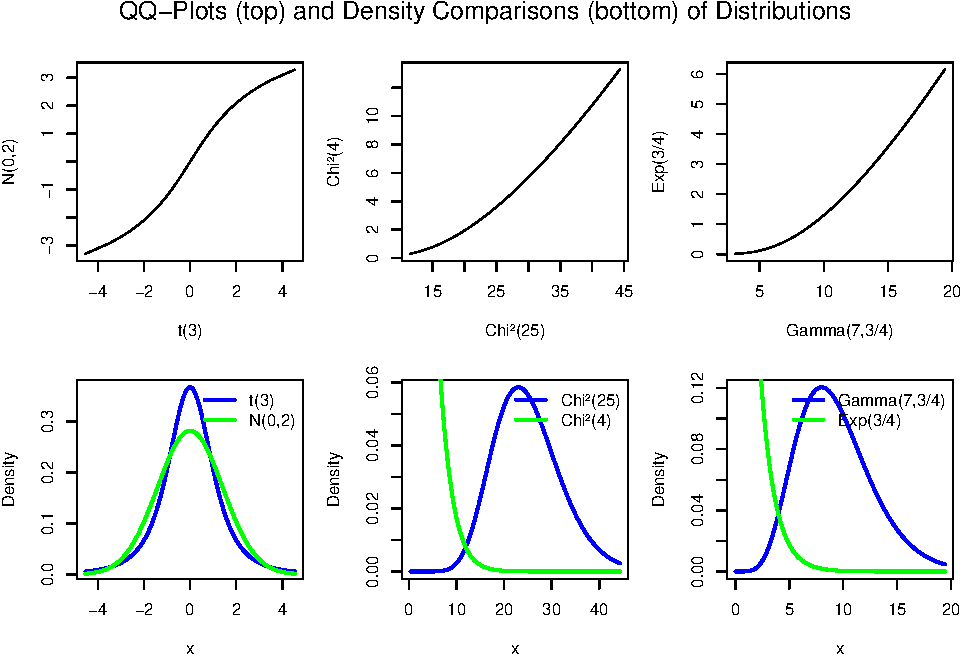
\includegraphics{SDA_A2_files/figure-latex/unnamed-chunk-1-1.pdf}

\subsection{b.}\label{b.}

\begin{Shaded}
\begin{Highlighting}[]
\CommentTok{\# Load necessary package}
\FunctionTok{library}\NormalTok{(EnvStats)}
\end{Highlighting}
\end{Shaded}

\begin{verbatim}
## 
## Attaching package: 'EnvStats'
\end{verbatim}

\begin{verbatim}
## The following objects are masked from 'package:stats':
## 
##     predict, predict.lm
\end{verbatim}

\begin{Shaded}
\begin{Highlighting}[]
\CommentTok{\# Read the data}
\NormalTok{mystery }\OtherTok{\textless{}{-}} \FunctionTok{readRDS}\NormalTok{(}\StringTok{"mysterious\_sample.RDS"}\NormalTok{)}

\CommentTok{\# Compute sample statistics}
\NormalTok{y\_bar }\OtherTok{\textless{}{-}} \FunctionTok{mean}\NormalTok{(mystery)  }\CommentTok{\# Sample mean}
\NormalTok{s\_y }\OtherTok{\textless{}{-}} \FunctionTok{sd}\NormalTok{(mystery)  }\CommentTok{\# Sample standard deviation}

\CommentTok{\# Define theoretical distribution parameters}
\CommentTok{\# 1. Uniform(0,1)}
\NormalTok{mu\_x\_unif }\OtherTok{\textless{}{-}}\NormalTok{ (}\DecValTok{0} \SpecialCharTok{+} \DecValTok{1}\NormalTok{) }\SpecialCharTok{/} \DecValTok{2}  \CommentTok{\# Mean of Uniform(0,1)}
\NormalTok{s\_x\_unif }\OtherTok{\textless{}{-}} \FunctionTok{sqrt}\NormalTok{((}\DecValTok{1} \SpecialCharTok{{-}} \DecValTok{0}\NormalTok{)}\SpecialCharTok{\^{}}\DecValTok{2} \SpecialCharTok{/} \DecValTok{12}\NormalTok{)  }\CommentTok{\# Standard deviation of Uniform(0,1)}
\NormalTok{b\_hat\_unif }\OtherTok{\textless{}{-}}\NormalTok{ s\_y }\SpecialCharTok{/}\NormalTok{ s\_x\_unif}
\NormalTok{a\_hat\_unif }\OtherTok{\textless{}{-}}\NormalTok{ y\_bar }\SpecialCharTok{{-}}\NormalTok{ b\_hat\_unif }\SpecialCharTok{*}\NormalTok{ mu\_x\_unif}

\CommentTok{\# 2. Extreme Value Distribution (EVD(0,1))}
\NormalTok{mu\_x\_evd }\OtherTok{\textless{}{-}} \FloatTok{0.5772}  \CommentTok{\# Mean of EVD(0,1)}
\NormalTok{s\_x\_evd }\OtherTok{\textless{}{-}} \FunctionTok{sqrt}\NormalTok{(pi}\SpecialCharTok{\^{}}\DecValTok{2} \SpecialCharTok{/} \DecValTok{6}\NormalTok{)  }\CommentTok{\# Standard deviation of EVD(0,1)}
\NormalTok{b\_hat\_evd }\OtherTok{\textless{}{-}}\NormalTok{ s\_y }\SpecialCharTok{/}\NormalTok{ s\_x\_evd}
\NormalTok{a\_hat\_evd }\OtherTok{\textless{}{-}}\NormalTok{ y\_bar }\SpecialCharTok{{-}}\NormalTok{ b\_hat\_evd }\SpecialCharTok{*}\NormalTok{ mu\_x\_evd}

\CommentTok{\# 3. Logistic(0,1)}
\NormalTok{mu\_x\_logis }\OtherTok{\textless{}{-}} \DecValTok{0}  \CommentTok{\# Mean of Logistic(0,1)}
\NormalTok{s\_x\_logis }\OtherTok{\textless{}{-}} \FunctionTok{sqrt}\NormalTok{(pi}\SpecialCharTok{\^{}}\DecValTok{2} \SpecialCharTok{/} \DecValTok{3}\NormalTok{)  }\CommentTok{\# Standard deviation of Logistic(0,1)}
\NormalTok{b\_hat\_logis }\OtherTok{\textless{}{-}}\NormalTok{ s\_y }\SpecialCharTok{/}\NormalTok{ s\_x\_logis}
\NormalTok{a\_hat\_logis }\OtherTok{\textless{}{-}}\NormalTok{ y\_bar }\SpecialCharTok{{-}}\NormalTok{ b\_hat\_logis }\SpecialCharTok{*}\NormalTok{ mu\_x\_logis}

\CommentTok{\# Print estimated slopes and intercepts}
\FunctionTok{cat}\NormalTok{(}\StringTok{"Estimated for Uniform(0,1): a ="}\NormalTok{, a\_hat\_unif, }\StringTok{", b ="}\NormalTok{, b\_hat\_unif, }\StringTok{"}\SpecialCharTok{\textbackslash{}n}\StringTok{"}\NormalTok{)}
\end{Highlighting}
\end{Shaded}

\begin{verbatim}
## Estimated for Uniform(0,1): a = -1.734457 , b = 14.00126
\end{verbatim}

\begin{Shaded}
\begin{Highlighting}[]
\FunctionTok{cat}\NormalTok{(}\StringTok{"Estimated for Extreme Value(0,1): a ="}\NormalTok{, a\_hat\_evd, }\StringTok{", b ="}\NormalTok{, b\_hat\_evd, }\StringTok{"}\SpecialCharTok{\textbackslash{}n}\StringTok{"}\NormalTok{)}
\end{Highlighting}
\end{Shaded}

\begin{verbatim}
## Estimated for Extreme Value(0,1): a = 3.447191 , b = 3.151391
\end{verbatim}

\begin{Shaded}
\begin{Highlighting}[]
\FunctionTok{cat}\NormalTok{(}\StringTok{"Estimated for Logistic(0,1): a ="}\NormalTok{, a\_hat\_logis, }\StringTok{", b ="}\NormalTok{, b\_hat\_logis, }\StringTok{"}\SpecialCharTok{\textbackslash{}n}\StringTok{"}\NormalTok{)}
\end{Highlighting}
\end{Shaded}

\begin{verbatim}
## Estimated for Logistic(0,1): a = 5.266175 , b = 2.22837
\end{verbatim}

\begin{Shaded}
\begin{Highlighting}[]
\CommentTok{\# Set up a 1x3 grid for plotting}
\FunctionTok{par}\NormalTok{(}\AttributeTok{mfrow =} \FunctionTok{c}\NormalTok{(}\DecValTok{1}\NormalTok{, }\DecValTok{3}\NormalTok{), }\AttributeTok{mar =} \FunctionTok{c}\NormalTok{(}\DecValTok{4}\NormalTok{, }\DecValTok{4}\NormalTok{, }\DecValTok{2}\NormalTok{, }\DecValTok{1}\NormalTok{), }\AttributeTok{oma =} \FunctionTok{c}\NormalTok{(}\DecValTok{0}\NormalTok{, }\DecValTok{0}\NormalTok{, }\DecValTok{2}\NormalTok{, }\DecValTok{0}\NormalTok{))}

\CommentTok{\# Generate QQ{-}Plots with Fitted Lines}

\CommentTok{\# 1. QQ{-}Plot: Sample vs Uniform(0,1)}
\FunctionTok{qqPlot}\NormalTok{(mystery, }\AttributeTok{distribution =} \StringTok{"unif"}\NormalTok{,}
       \AttributeTok{param.list =} \FunctionTok{list}\NormalTok{(}\AttributeTok{min =} \DecValTok{0}\NormalTok{, }\AttributeTok{max =} \DecValTok{1}\NormalTok{),}
       \AttributeTok{add.line =} \ConstantTok{FALSE}\NormalTok{, }\AttributeTok{main =} \StringTok{""}\NormalTok{,}
       \AttributeTok{xlab =} \StringTok{"Theoretical Quantiles }\SpecialCharTok{\textbackslash{}n}\StringTok{ (Uniform(0,1))"}\NormalTok{,}
       \AttributeTok{ylab =} \StringTok{"Sample Quantiles"}\NormalTok{)}
\FunctionTok{abline}\NormalTok{(}\AttributeTok{a =}\NormalTok{ a\_hat\_unif, }\AttributeTok{b =}\NormalTok{ b\_hat\_unif, }\AttributeTok{col =} \StringTok{"red"}\NormalTok{, }\AttributeTok{lwd =} \DecValTok{2}\NormalTok{)  }\CommentTok{\# Add fitted line}

\CommentTok{\# 2. QQ{-}Plot: Sample vs Extreme Value(0,1)}
\FunctionTok{qqPlot}\NormalTok{(mystery, }\AttributeTok{distribution =} \StringTok{"evd"}\NormalTok{,}
       \AttributeTok{param.list =} \FunctionTok{list}\NormalTok{(}\AttributeTok{location =} \DecValTok{0}\NormalTok{, }\AttributeTok{scale =} \DecValTok{1}\NormalTok{),}
       \AttributeTok{add.line =} \ConstantTok{FALSE}\NormalTok{, }\AttributeTok{main =} \StringTok{""}\NormalTok{,}
       \AttributeTok{xlab =} \StringTok{"Theoretical Quantiles }\SpecialCharTok{\textbackslash{}n}\StringTok{ (EVD(0,1))"}\NormalTok{,}
       \AttributeTok{ylab =} \StringTok{" "}\NormalTok{)}
\FunctionTok{abline}\NormalTok{(}\AttributeTok{a =}\NormalTok{ a\_hat\_evd, }\AttributeTok{b =}\NormalTok{ b\_hat\_evd, }\AttributeTok{col =} \StringTok{"red"}\NormalTok{, }\AttributeTok{lwd =} \DecValTok{2}\NormalTok{)  }\CommentTok{\# Add fitted line}

\CommentTok{\# 3. QQ{-}Plot: Sample vs Logistic(0,1)}
\FunctionTok{qqPlot}\NormalTok{(mystery, }\AttributeTok{distribution =} \StringTok{"logis"}\NormalTok{,}
       \AttributeTok{param.list =} \FunctionTok{list}\NormalTok{(}\AttributeTok{location =} \DecValTok{0}\NormalTok{, }\AttributeTok{scale =} \DecValTok{1}\NormalTok{),}
       \AttributeTok{add.line =} \ConstantTok{FALSE}\NormalTok{, }\AttributeTok{main =} \StringTok{""}\NormalTok{,}
       \AttributeTok{ylab =} \StringTok{" "}\NormalTok{,}
       \AttributeTok{xlab =} \StringTok{"Theoretical Quantiles }\SpecialCharTok{\textbackslash{}n}\StringTok{ (logistic(0,1))"}\NormalTok{)}
\FunctionTok{abline}\NormalTok{(}\AttributeTok{a =}\NormalTok{ a\_hat\_logis, }\AttributeTok{b =}\NormalTok{ b\_hat\_logis, }\AttributeTok{col =} \StringTok{"red"}\NormalTok{, }\AttributeTok{lwd =} \DecValTok{2}\NormalTok{)  }\CommentTok{\# Add fitted line}

\CommentTok{\# {-}{-}{-} Add an Overall Title {-}{-}{-}}
\FunctionTok{mtext}\NormalTok{(}\StringTok{"QQ{-}Plots in comparing sample quantiles to the theoretical quantiles"}\NormalTok{, }\AttributeTok{outer =} \ConstantTok{TRUE}\NormalTok{, }\AttributeTok{cex =} \DecValTok{1}\NormalTok{, }\AttributeTok{font =} \FloatTok{0.5}\NormalTok{)}
\end{Highlighting}
\end{Shaded}

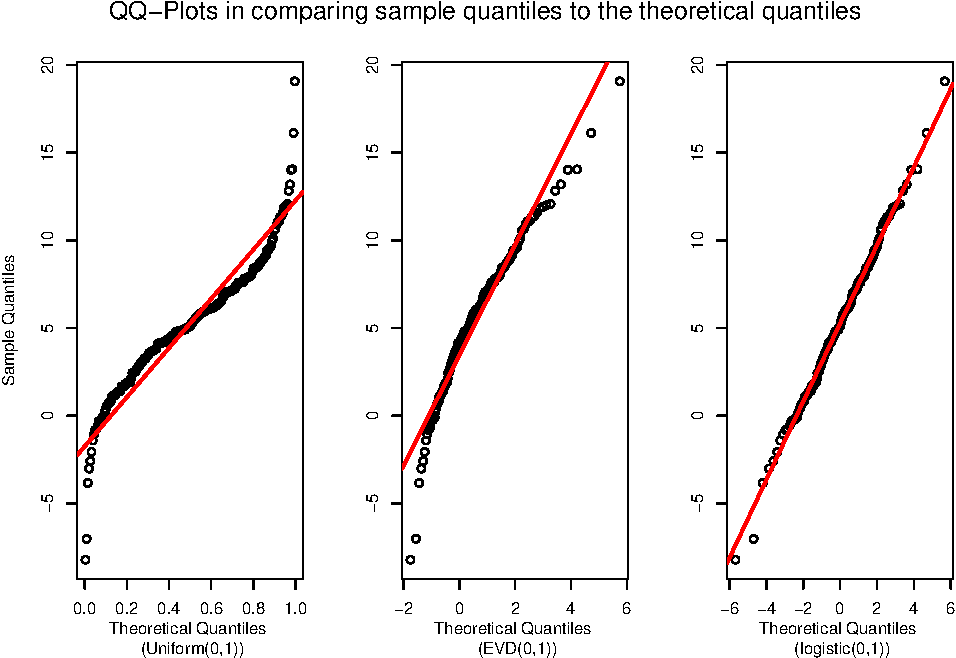
\includegraphics{SDA_A2_files/figure-latex/unnamed-chunk-2-1.pdf} In the
plot, the black circles are points of sample quantiles plotted against
theoretical quantiles, and the red lines are fitted line given those
points with parameter a (intercept) and b (slope). As can be seen from
the qq-plots, the logistic distribution fits the data the best because
the qq-plot almost looks like a straight line. the other two qq-plots
are more curvy and have tails. Estimated for Uniform(0,1): a = -1.734457
, b = 14.00126 Estimated for Extreme Value(0,1): a = 3.447191 , b =
3.151391 Estimated for Logistic(0,1): a = 5.266175 , b = 2.22837

\section{Exercise 2}\label{exercise-2}

\subsection{a.}\label{a.-1}

\begin{Shaded}
\begin{Highlighting}[]
\CommentTok{\# load dataset}
\NormalTok{parakeets }\OtherTok{\textless{}{-}} \FunctionTok{readRDS}\NormalTok{(}\StringTok{"parakeets.RDS"}\NormalTok{)}

\CommentTok{\# select the list of weights where the year is 1980 and 2015 respectively}
\NormalTok{parakeet\_weights\_1980 }\OtherTok{\textless{}{-}}\NormalTok{ parakeets}\SpecialCharTok{$}\NormalTok{Weight[parakeets}\SpecialCharTok{$}\NormalTok{Year }\SpecialCharTok{==} \DecValTok{1980}\NormalTok{]}
\NormalTok{parakeet\_weights\_2015 }\OtherTok{\textless{}{-}}\NormalTok{ parakeets}\SpecialCharTok{$}\NormalTok{Weight[parakeets}\SpecialCharTok{$}\NormalTok{Year }\SpecialCharTok{==} \DecValTok{2015}\NormalTok{]}

\CommentTok{\# set the grid to 1x2 for plotting the histograms}
\FunctionTok{par}\NormalTok{(}\AttributeTok{mfrow =} \FunctionTok{c}\NormalTok{(}\DecValTok{1}\NormalTok{, }\DecValTok{2}\NormalTok{))}
    
\CommentTok{\# plotting for 1980}
\FunctionTok{hist}\NormalTok{(parakeet\_weights\_1980, }\AttributeTok{xlim =} \FunctionTok{c}\NormalTok{(}\DecValTok{100}\NormalTok{, }\DecValTok{140}\NormalTok{), }\AttributeTok{main =} \StringTok{"Weight Distribution (1980)"}\NormalTok{, }
     \AttributeTok{xlab =} \StringTok{"Weight (g)"}\NormalTok{)}

\CommentTok{\# plotting for 2015}
\FunctionTok{hist}\NormalTok{(parakeet\_weights\_2015, }\AttributeTok{xlim =} \FunctionTok{c}\NormalTok{(}\DecValTok{100}\NormalTok{, }\DecValTok{140}\NormalTok{), }\AttributeTok{main =} \StringTok{"Weight Distribution (2015)"}\NormalTok{, }
     \AttributeTok{xlab =} \StringTok{"Weight (g)"}\NormalTok{)}
\end{Highlighting}
\end{Shaded}

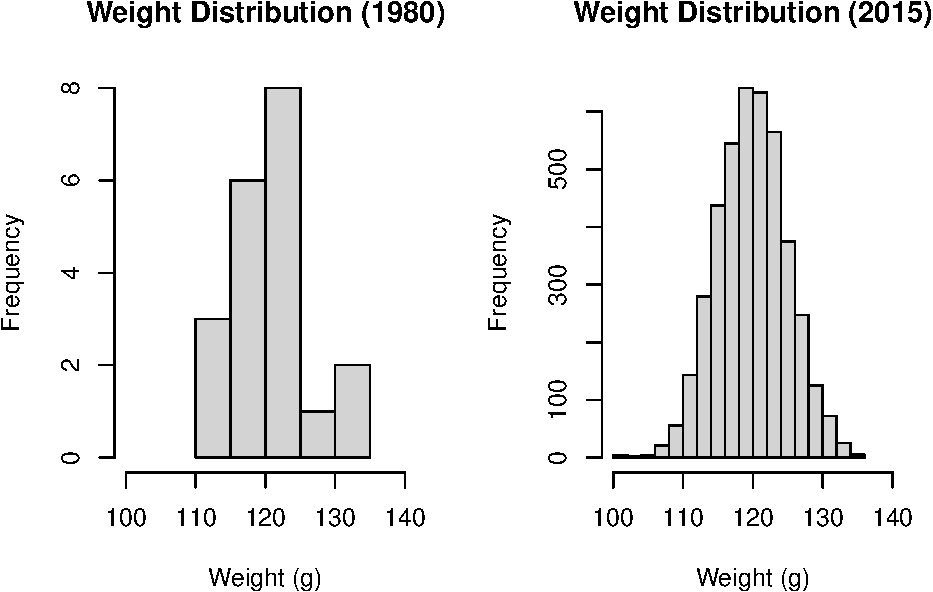
\includegraphics{SDA_A2_files/figure-latex/unnamed-chunk-3-1.pdf} The
underlying distributions could be the same since the peak is at around
the same weight, but this is hard to say since 1980 only has 20 samples.

\subsection{b.}\label{b.-1}

\begin{Shaded}
\begin{Highlighting}[]
\FunctionTok{qqplot}\NormalTok{(parakeet\_weights\_1980, parakeet\_weights\_2015, }
       \AttributeTok{main =} \StringTok{"QQ{-}Plot: 1980 vs 2015 Parakeet Weights"}\NormalTok{,}
       \AttributeTok{xlab =} \StringTok{"1980 Weights"}\NormalTok{, }
       \AttributeTok{ylab =} \StringTok{"2015 Weights"}\NormalTok{)}

\CommentTok{\# Add a reference line}
\FunctionTok{abline}\NormalTok{(}\DecValTok{0}\NormalTok{, }\DecValTok{1}\NormalTok{, }\AttributeTok{col =} \StringTok{"red"}\NormalTok{, }\AttributeTok{lwd =} \DecValTok{2}\NormalTok{)}
\end{Highlighting}
\end{Shaded}

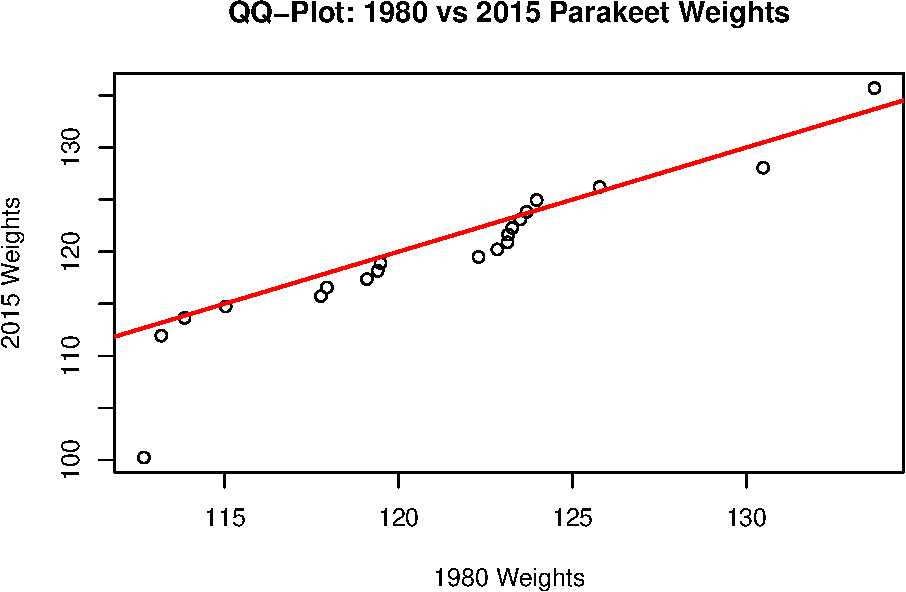
\includegraphics{SDA_A2_files/figure-latex/unnamed-chunk-4-1.pdf} The
points approximately follow the reference line so the distributions have
the same shape. Thus they could be the same location-scale family
(looking at the 2015 weight histogram they are probably both normal
distributions). \#\# c.

\begin{Shaded}
\begin{Highlighting}[]
\CommentTok{\# set the grid to 1x2 for plotting the QQ{-}plots}
\FunctionTok{par}\NormalTok{(}\AttributeTok{mfrow =} \FunctionTok{c}\NormalTok{(}\DecValTok{1}\NormalTok{,}\DecValTok{2}\NormalTok{))}

\CommentTok{\# QQ{-}Plot for 1980 Weights}
\FunctionTok{qqnorm}\NormalTok{(parakeet\_weights\_1980, }\AttributeTok{main =} \StringTok{"QQ{-}Plot: Normal (1980)"}\NormalTok{)}
\CommentTok{\# Add a reference line}
\FunctionTok{qqline}\NormalTok{(parakeet\_weights\_1980, }\AttributeTok{col =} \StringTok{"red"}\NormalTok{, }\AttributeTok{lwd =} \DecValTok{2}\NormalTok{)}

\CommentTok{\# QQ{-}Plot for 2015 Weights}
\FunctionTok{qqnorm}\NormalTok{(parakeet\_weights\_2015, }\AttributeTok{main =} \StringTok{"QQ{-}Plot: Normal (2015)"}\NormalTok{)}
\CommentTok{\# Add a reference line}
\FunctionTok{qqline}\NormalTok{(parakeet\_weights\_2015, }\AttributeTok{col =} \StringTok{"red"}\NormalTok{, }\AttributeTok{lwd =} \DecValTok{2}\NormalTok{)}
\end{Highlighting}
\end{Shaded}

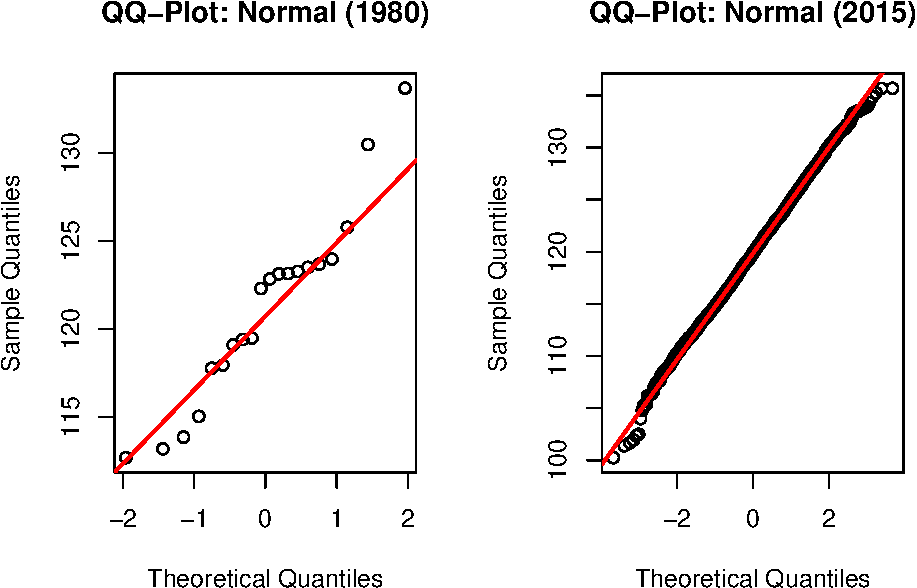
\includegraphics{SDA_A2_files/figure-latex/unnamed-chunk-5-1.pdf} The
weights from the 2015 sample seem to very clearly follow a normal
distribution. The weights from the 1980 sample seem the deviate a little
more from the fitted line, but they still follow it so it probably still
originates from a normal distribution. The 1980 sample needs more
weights to get more confidence in this conclusion.

\subsection{d.}\label{d.}

\begin{Shaded}
\begin{Highlighting}[]
\NormalTok{shapiro\_1980 }\OtherTok{\textless{}{-}} \FunctionTok{shapiro.test}\NormalTok{(parakeet\_weights\_1980)}
\NormalTok{shapiro\_2015 }\OtherTok{\textless{}{-}} \FunctionTok{shapiro.test}\NormalTok{(parakeet\_weights\_2015)}

\FunctionTok{print}\NormalTok{(shapiro\_1980)}
\end{Highlighting}
\end{Shaded}

\begin{verbatim}
## 
##  Shapiro-Wilk normality test
## 
## data:  parakeet_weights_1980
## W = 0.94612, p-value = 0.312
\end{verbatim}

\begin{Shaded}
\begin{Highlighting}[]
\FunctionTok{print}\NormalTok{(shapiro\_2015)}
\end{Highlighting}
\end{Shaded}

\begin{verbatim}
## 
##  Shapiro-Wilk normality test
## 
## data:  parakeet_weights_2015
## W = 0.99919, p-value = 0.0496
\end{verbatim}

The Null hypothesis isn't rejected for the 1980 sample since the p-value
is more than 0.05 (corresponding to the significance level of 5\%) which
doesn't mean that it is normally distributed but it says that we don't
have significant proof that it isn't normally distributed. The Null
hypothesis for the the 2015 sample is rejected since the p-value of
0.0496 is lower than 0.05. This means we have significant proof that the
2015 sample isn't normally distributed.

\subsection{e.}\label{e.}

In the graphs for the 1980 sample we couldn't say for sure that it
followed a normal distribution, but it looked like it did and the
Shapiro-Wilk normality test said that it is either normal or we don't
have enough data to be confident that it isn't normal. Thus the
conclusion is that the 1980 sample is probably follows a normal
distribution but it is inconclusive because of the small sample size.
The graphs for the 2015 sample show that it follows a normal
distribution. The Shapiro-Wilk normality test says that the sample isn't
normal, but this test is more sensitive to small deviations from a
normal distribution as the sample size increases and from the graphs you
can see that this probably happens due to the tails that deviate from a
normal distribution. Thus the 2015 sample doesn't follow a normal
distribution exactly, but the distribution that it follows can be
approximated really well by a normal distribution, especially in the
area exclusing the tails.

\end{document}
